\documentclass{article} 
\usepackage{graphicx}
\usepackage{geometry,amssymb,amsmath,listings,float,blindtext}
\geometry{
 a4paper,
 total={170mm,257mm},
 left=20mm,
 top=20mm,
 }

\linespread{1.5}
\title{The Matchmakers: Data Analysis Report}

\author{
  D'Azevedo, Gloria\\
  \texttt{gad87@cornell.edu}
  \and
  Yadav, Pihu\\
  \texttt{py82@cornell.edu}
}
\date{December 5, 2016}

\begin{document}
\maketitle

\section{Executive Summary}
The goal of this analysis is to create a model that identifies whether or not a male and a female are a match in the speed dating context. The main aim of the project is to develop a model, that will identify important traits people look for in a partner so that effective onboarding surveys for speed dating events or online dating will have high accuracy rates in predicting matches. This would allow speed dating event organisers and online dating apps to give better recommendations to users for partners and would answer important questions that most people have in their dating lives, such as what potential partners are looking for.  The data has several types of formats including ordinal variables, open ended text variables, and binary variables.  The 3 types of models that are tested are a nonregularized linear model using best subset selection, two logistic models, and a regularized model using lasso with cross-validation.  Some analysis was also done using the unsupervised method K-Nearest-Neighbors but the misclassification rates were very high so our current implementation and predictors used is not the best for this problem.  In the future we hope to incorporate other variables indicative of a ``match" such as one person calling the other or the two people going on a date.  However, these fields, that were covered in surveys taken after the speed dating exercise, have low response rates and a high bias so they may not be completely reliable but could still give good insights about the data if we had more responses. 

\section{Introduction}
%Problem: 
The main goal of this analysis is to develop a model that predicts whether or not two people (a male and a female) will be attracted to one another.  We want to do this by identifying what traits individuals look for and value most in their partners. Some obvious applications for this model will be organizing future speed dating events as well as online surveys that online dating websites or mobile applications use to determine potential matches for a participant. The ideal model should work on both genders, and the model should be sparse or relatively small so that the surveys and forms (where we get data) will be shorter so people are more likely to complete the whole thing truthfully when prompted.\\
\null\\
The data used in the analysis is the Kaggle Speed Dating Experiment data set which was obtained from speed dating events conducted by Columbia Business School professors.  (https://www.kaggle.com/annavictoria/speed-dating-experiment). There are 21 different speed dating events (waves) that occur between October 2002 and April 2004, each of which have between 10 and 45 participants, and the number of men and women are roughly equal in each.  Each participant is asked to fill out a total of 4 surveys in addition to questionnaires about their partners during the events.  The first survey occurs when they sign up, the second is halfway through the speed dating event, the third is the first follow-up the day after the speed dating event so that they will get a list of their matches, and the fourth is the second follow-up after the speed dating event which is sent 3-4 weeks after they had been sent their matches. However, it is important to note that the response rates for each of the 4 surveys are not 100\% and the missing data poses a huge problem for some of the algorithms.\\
\null\\
The types of questions asked on the survey are mostly ordinal or categorical variables with a couple of open-ended text questions.  Some of the open ended questions have a low completion response rate such as the age field and also the school that you completed your undergraduate degree.  These fields therefore cannot be reliably used in the analysis because there could be inherent biases for why the participants did not respond. In the future, surveys can still ask these types of questions as a categorical or multiple-choice variable by giving participants a few age ranges that they can choose from so they would not be explicitly stating their age (a potential reason for nonresponse). 
%
\section{Data Cleaning Remarks}
\label{sec:dataclean}
During the following report we will take on the convention that a ``participant" is the person filling out the survey and the ``partner" is the person they interact with during that particular round of the speed dating wave.  When scraping data and analyzing the coefficients of the predictors in the model, we denote the ``participant" as the female and the ``partner" as the male, so that the data is not double counted.  All females have interacted with each male once and vice versa so this is not a problem.  There is only one incident of a person not completing her initial surveys.\\
%\null\\
%Some cities and jobs in the data had commas in the open ended responses, so we had to remove the commas as otherwise the import would not work correctly and would break up all those fields and not import the correct value per column or the correct number of columns.  The apostrophe's caused a similar problem so they were either removed or the word was rewritten so that it would not need to be shortened with an apostrophe (i.e. changing ``Int'l" to ``International").  In general, these columns were not used in the analysis from the ambiguous responses and low response rates but they would break the import.\\
%\null\\
%There were some blanks in the "pid" field that corresponded to the partner's id of the current participant for some of the id's in Wave 5. We deduced that the 7th female  didn't complete her responses to either the first survey or to the first follow up survey. Thus, we assume that she did not match with anyone and assign the "dec" and "dec\_0" fields which correspond to her decision to be 0. We chose not to delete all the corresponding rows entirely since they have information about male preferences for not matching with her.\\
%\null\\
%For the "int\_corr" field which is defined in the key as the correlation between the participant and the partner's ratings of interesting Time 1, we substitute the blanks for 0's to indicate that there is no correlation as we are not sure how the field is exactly calculated. If we decide to use a similar field, we can insert a new "correlation" column at the end of the data where we know the calculation deterministically.\\
\null\\
For many questions in all the surveys, participants are asked in the surveys to divide up 100 points to 6 attributes by importance.  These main 6 attributes are attractivness, sincerity, intelligence, fun personality, ambition, and shared interests.  However, there are several questions where the shared interests are either not recorded in our data or the survey forgot that attribute when asking the participant.  It may be possible to impute that value for some participants if we assume that the question was asked on the survey but the data is not recorded by subtracting the sum of the points for the other attributes from 100 to get the points for the shared interests attribute as long as there is no non-response in the other questions.\\
%\null\\
%Some fields are inter-related so if there are blank values in one of them, then the value cannot be found in the similar field. For example, there are two fields ``age\_o" and ``age". ``Age" is the self-reported age of the student and is asked when they signed up. ``age\_o" is the age of the partner during that round.  The values for ``age\_o" must have inputted after the survey was asked.  For example, if a participant did not report her age, the value for ``age\_o" for all the partners she had are also null.  The problem with age is that there are many possibilities why people did not report their true age.  For example, men tend to like young women, so women may report a lower age than the true value.  On the other hand, women prefer older, mature men as a measure of stability so men may report a higher age than the true value.  For now we did not edit or add any of the ``age" or ``age\_o" values, nor do we use them in the analysis but when we have to impute variables to implement the K-Nearest-Neighbors (KNN) on the data, then we use the average age of the non-blank variables into the blank and NA values.\\
\null\\
While investigating trends in categorical data such as the ``field\_cd" column (corresponds to a numerical code for the field of study that each person has) or ``race" (integer corresponding to a type of race), we noted that there were some NA values so we reassigned those NA values to be that predictor's ``Other" category.  Even though we would be over-counting the trends in the ``Other" category, we hope that the majority of participants had accurately written down their race or what field they classify themselves in.  If the data field was an ordinal variable such as ``tv" (measures the interest that a person has in watching TV on a scale from 1 to 10) we can reassign NA values to be 0, indicating that they had no interest in that activity and that's why the participants left them blank.  Obviously, imputing too much data affects the results significantly, so we only do that when trying to implement the KNN algorithm in Section \ref{sec:KNN}.\\
%\null\\
%Some of the survey fields requires a participant to rate their preferences about their partner; however, there are different instructions for this variable on the survey for different waves.  For example, during the initial survey before the events took place, the participants in waves 1-5 and 10-21 were asked to divide up 100 points among 6 different categories (more points implies higher importance).  In contrast, the participants in waves 6-9 were asked to rate each category on a scale of 1-10 for the importance of each attribute in a partner (a rating of 1 indicates that the attribute is not at all important while a rating of 10 is extremely important).  When we investigated the data by wave, the participants in waves 6-9 have also divided weights from 100 into the 6 attributes even though the key or instructions have said otherwise. Since each of the attribute weights are all on the same scale for all waves, the values did not need to be normalize the weights to the same scale.
%\null\\
%For some of the analyses, the NA values were reassigned to be zeroes so that numerical calculations and the machine learning algorithm can be performed although we also note that usually if there were NA values in one attribute, the other 5 attributes in that section were also missing.  There are many other fields that have weights or ranks as the expected input, so if the fields were not completed, (i.e. the participant left the field blank) then we reassign those blanks or NA values to be 0 indicating that the field is not important to them.
%
\section{Initial Data Analysis and Methods}
%For some of the fields, the survey asks the participant what they think how other people rank several traits. However, it may not be that important to know what the participant thinks that other people prefer.  It is better to look at actual proof of what people value based on the traits of people that they liked during the speed dating event, regardless of whether or not the other person liked them back.  \\
%\null\\
%Importance of activities: 
In the initial sign-up survey, participants are asked how important each of 17 different activities are to them.  The activities include yoga, reading, and watching sports, and there may be high correlation between the interest level in some of the activities.  For example, a person who likes theater may also really enjoy watching movies.  These values are integer values from 0 to 10 and a higher value implies higher interest in the activity. \\ %If two people have similar amounts of interest in the activity, then that should reflect in their classifications assuming that the participants do not mis-rank the interest level. We hypothesize that including similar levels of key interests should improve accuracy of classification.\\  
\null\\
We tried fitting a linear model predicting match with all of the activities for both men and women (total of 34 variables) and taking only the significant variables from those to get a model.  In addition, we try using a forward/backward selection algorithm using AIC to find an optimal model using the activities.  Unfortunately we did not see that the same activities for both men and women were chosen so in the implementation we would have to have different onboarding surveys for men and women or we would include the nonsignificant variables on both surveys for the sake of consistency.  We also considered using a vector of absolute differences ($||\cdot||_1$) or the sum of squared differences ($||\cdot||_2^2$) between the interest level in an activity between two people. \\
\null\\
In one analysis, we want to identify how men value different traits that they want in a partner. Initially we computed the summary statistics for all the entries where men said 'yes' to their partner. This helped in getting a broad overview of the problem as it gave us the mean, median, maximum, minimum and some quantile values for the parameters we are interested in such as the scores given by the male participant for attributes such as attractiveness, sincerity, intelligience etc. to the partners they said 'yes' to. This helped us in getting an overall idea of what traits men value highly as high average or median scores in a particular category generally meant that men valued that trait. However, comparing summary values is not an adequate indicator of the significance of certain predictors, so we later develop a more detailed model. \\
\begin{table}[!htbp] \centering 
  \caption{Summary table for key statistics} 
  \label{fig:sum_table} 
\begin{tabular}{@{\extracolsep{5pt}}lccccc} 
\\[-1.8ex]\hline 
\hline \\[-1.8ex] 
Statistic & \multicolumn{1}{c}{N} & \multicolumn{1}{c}{Mean} & \multicolumn{1}{c}{St. Dev.} & \multicolumn{1}{c}{Min} & \multicolumn{1}{c}{Max} \\ 
\hline \\[-1.8ex] 
Same Race & 3,518 & 0.409 & 0.492 & 0 & 1 \\ 
Attractiveness & 3,507 & 7.285 & 1.533 & 1 & 10 \\ 
Sincerity & 3,480 & 7.596 & 1.514 & 0 & 10 \\ 
Intelligence & 3,474 & 7.757 & 1.330 & 3 & 10 \\ 
Fun & 3,449 & 7.334 & 1.512 & 0 & 10 \\ 
Ambition & 3,271 & 7.159 & 1.592 & 0 & 10 \\ 
Shared Interests & 3,167 & 6.463 & 1.841 & 0 & 10 \\ 
\hline \\[-1.8ex] 
\end{tabular} 
\end{table} 
%
We also plotted the scores given to partners for different characteristics, along with whether the participant said 'yes' to them. This plays a strong role in understanding whether high scores for a particular attribute correspond to more 'yes''s than 'no''s, which means that it is am important trait that people value in their partners. Attractiveness scores are later found to be a strong attribute for predicting the decision of a participant and we see from the graph below that partners who were given low attractiveness scores generally get more 'no''s whereas partners with high attractiveness scores get more 'yes''s.\\
\begin{figure}[H]
	\caption{Histogram of Attractiveness Scores}
	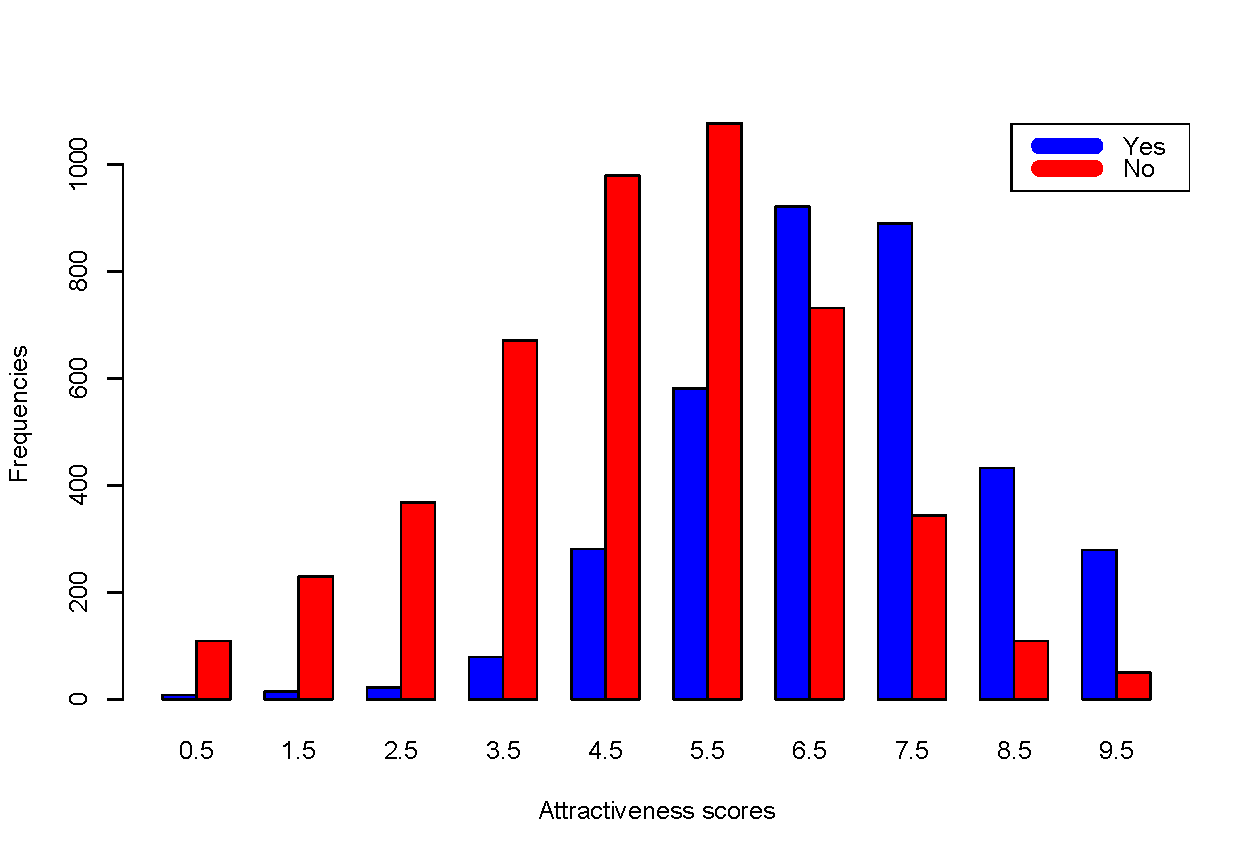
\includegraphics[scale=0.50]{AttractivenessScores}
	\centering
	\label{fig:attractiveness}
\end{figure}
%Rather than considering the priorities assigned to the individual parameters, we choose to compare the values of scores given to partners they said `yes' to with the scores of all the partners. Initially we computed the summary statistics to get a broad idea of the difference between the two. Following this we performed a linear regression on the decision variable (dec) to determine which of the different parameters had the greatest impact on its value. The results of the regression suggest that while perceived attractiveness, sincerity, `fun-ness', ambition and shared interests do play a role in deciding a man's decision, other factors such as intelligence, the partner being of the same race and actual shared interests do not play a major role.
\section{Model Development}
\subsection{Logistic Regression}
\label{sec:logistic}
We want to identify how men value different attributes that they want in a partner (attractiveness, sincerity, intelligence, being fun, ambition and shared interests). This is part of our attempts to understand gender differences in what participants look for in a partner. We also include the parameter ``samerace" (which identifies whether the partner is of the same race) in the analysis.\\
\null\\
Since the decision variable (of saying `yes' or `no' to a partner) is boolean we have chosen to use logistic regression for the analysis. The variables used include the scores given to partners (for attractiveness, sincerity, intelligence etc.) and whether or not the partner and the participant are of the same race. The results of this preliminary analysis suggested that attractiveness, sincerity, being fun, ambition and having shared interests are significant in a man's decision and intelligence and being of the same race are not significant. Of these significant parameters: attractiveness, being fun and having shared interests are positively correlated with the final decision, but sincerity and ambition are negatively correlated with the male's decision. In this analysis all the values with missing data have been removed from the data when computing the coefficients for the logistic regression, as it would be misleading to impute the values of scores given to partners or assign the average value when the answer has been left blank by the participant. We do not expect this to create problems in our analysis since more than 75\% of the data is still available. \\
\null\\
In another analysis we incorporate the priorities assigned by participants to the weights assigned to the 6 main characteristics as well as their interaction effects with their partner's rating.  Interaction effects in the linear regression setting refer to the product of the two variables, multiplying the score for a parameter with its associated importance, gives us a new value for each of the parameters. There should be a direct correlation between the new scores given to a partner and the final decision (`yes' or `no').  Hence, our model is able to predict the most important factors in determining the final decision of a participant. 
The logistic regression shows that the interaction between partner attractiveness and priority of attractiveness, sincerity, and several other factors are significant in determining a participant's decision.  Other parameters such as intelligence and being fun are not significant to the model. It is interesting to see that while in the previous analysis, partners being of the same race was not found to be significant, in this analysis the interaction between the variable for the importance of a partner being of the same race and the variable identifying whether the partners are of the same race was found to be highly significant to the model. This means that while, from an overall perspective, partners having the same race was not found to be significant, in cases where the participant said having a partner of the same race was important to them, it became significant.
%
\subsection{Best Subset Selection Using Linear Models}
\label{sec:bestsubsetsection}
We have also implemented the best subset selection model using exhaustive search, which studies all combinations of predictors for a given model size.  For this analysis we estimate the decision that a participant gives their partner by using the main 6 variables (detailed in Section \ref{sec:dataclean}) as well as other variables such as how much they liked the partner, the probability with which they think their partner will say yes to them, how happy they expect to be with the speed dating exercise, how often they go out (to see if extroverted behavior correlates with saying yes to more people), their goal behind attending the speed dating exercise, whether they have met the partner before and how often they go on dates. We have taken care to include only the variables that could directly impact outcome and have disregarded those that have a large number of missing values. \\
\null\\
The best subset in our model is selected using the Bayesian Information criterion (BIC) which is a criterion that uses both the maximum likelihood value as well as the number of parameters in the model to determine the best model overall. Thus, it takes into account how accurately the model fits the data while at the same time penalising models that have a large number of parameters. Hence, when determining the best model overall model, it gives us an accurate as well as a simple model.\\
\null\\
For a model containing a single predictor, the best one was found to be the score given for how much they liked the partner, this is clearly understandable as how much you like a person should have a very strong correlation with whether you say yes to them. For a model with two predictors, the best possible combination was found to be the score for how much they liked the partner and the score they gave for attractiveness of the partner. This is also clearly justifiable. Similarly, best possible subset combinations were predicted for subsets containing just one variable to those containing all thirteen variables. The best subset among all possible combinations of predictors and number of predictors was found to be the one containing 9 variables, which were the scores given to the partner for attractiveness, sincerity, being fun, ambitious, having shared interests as well as how much they liked the partner, the probability with which they expect their partner to say yes to them, the score for how often they go out and the one for how happy they expect to be with the speed dating exercise.  The corresponding misclassification rate for this model is $\approx$ 24\%.\\
\null\\
While most of the predictors such as attractiveness, sincerity etc. are easy to justify, it is interesting to see that participants were more likely to say yes to a partner when they thought it was highly probable that their partner would say yes to them. Also, participants who go out more often were also likely to say yes to more partners and those who expected to be happy with the speed dating exercise also said yes to more people. This indicates the possibility of a feedback loop, so participants who expect the speed dating exercise to go well for them are able to find more people that they are interested in.
%\begin{figure}[H]
%	\caption{Results from Best Subset Selection for model size up to 13}
%	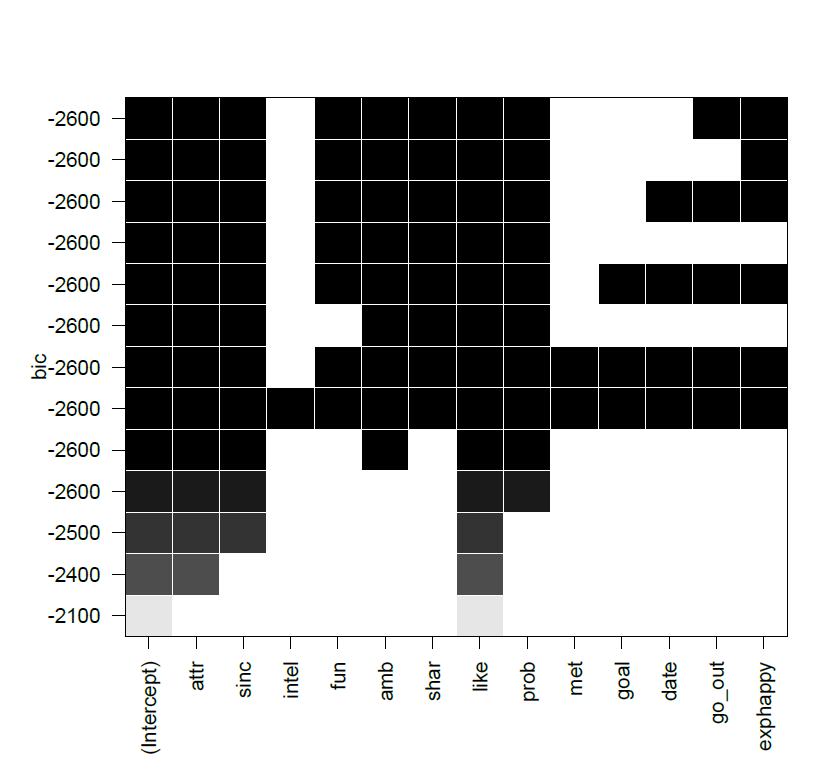
\includegraphics[scale=0.60]{bestsubsets}
%	%\centering
%	\label{fig:bestsubset}
%\end{figure}
%\begin{figure}[H]
%	\caption{BIC values for the best subsets}
%	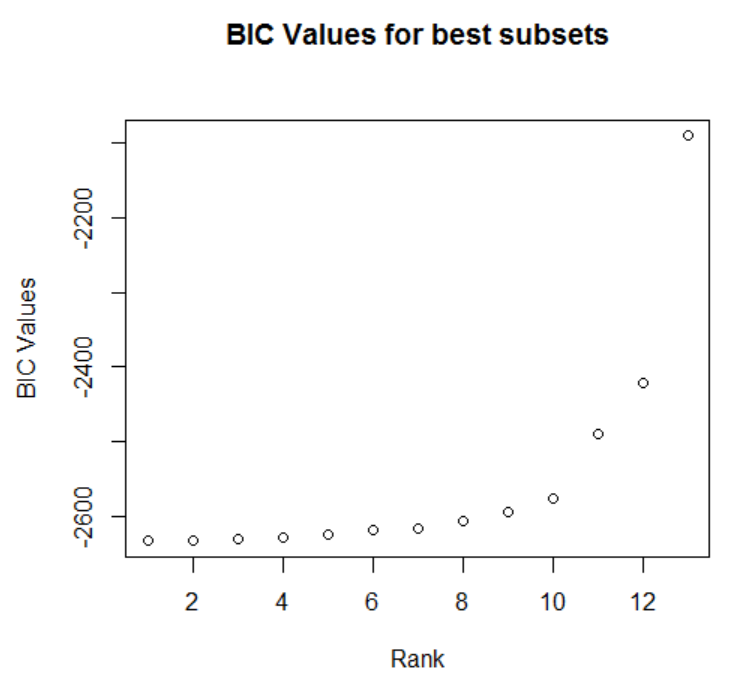
\includegraphics[scale=0.60]{BIC_sort}
%	%\centering
%	\label{fig:BICsort}
%\end{figure}

\begin{figure}[H]
	\centering
	\begin{minipage}{0.45\textwidth}
		\centering
		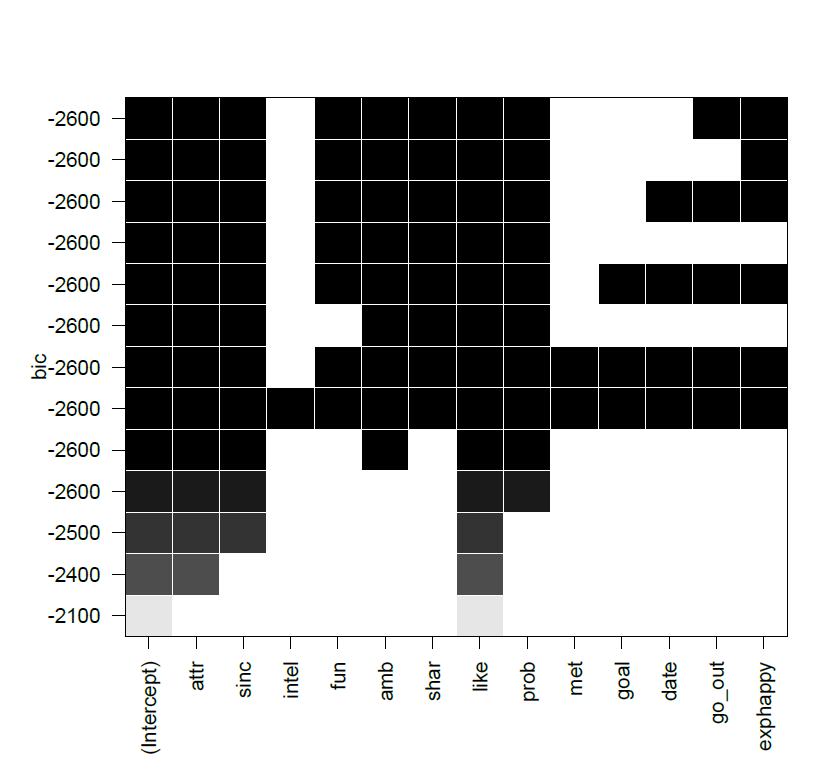
\includegraphics[width=0.9\textwidth]{bestsubsets} % first figure itself
		\caption{Results from Best Subset Selection for model size up to 13}
		\label{fig:bestsubsets}
	\end{minipage}\hfill
	\begin{minipage}{0.45\textwidth}
		\centering
		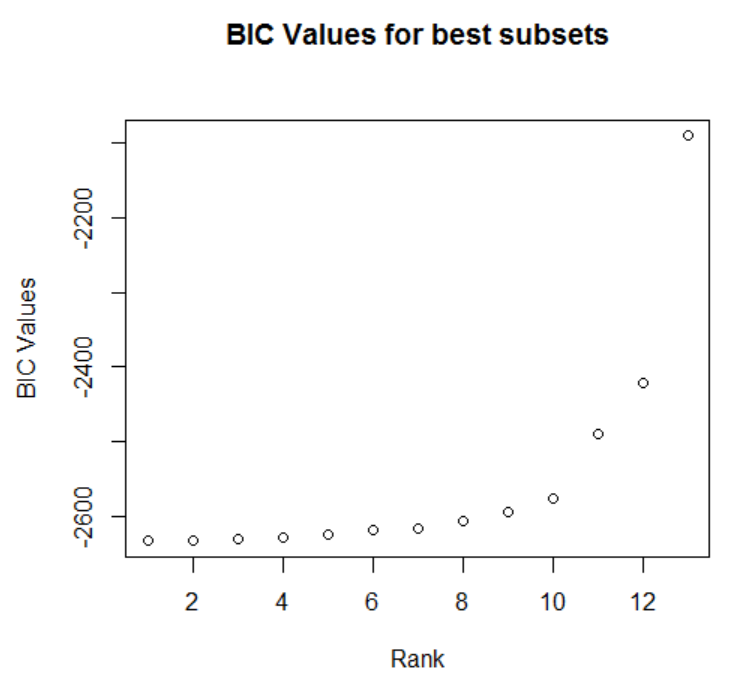
\includegraphics[width=0.9\textwidth]{BIC_sort} % second figure itself
		\caption{BIC values for the best subsets}
		\label{fig:BICsort}
	\end{minipage}
\end{figure}

In Figure \ref{fig:bestsubsets}, the BIC values for the top 10 models look to be about the same.  However, explicitly calculating them for each of the model sizes in Figure \ref{BICsort}, we can see that the top 5 models have BIC within a margin of 10 so they are all very good fits and the top model of size 9 has essentially the same BIC value as the second best model of size 8 so if we wanted to further decrease variance but not sacrifice fit, we could also use the second best model.
%
\subsection{Cross-Validation with Lasso Regularizer}
In the logistic regression models described in Section \ref{sec:logistic}, we used the entire dataset to create our model.  While this creates a comprehensive model, it may not predict new data accurately.  One way to estimate test error is to perform cross-validation, a technique that picks the best model on the basis of how well it performs when tested on the data it has not trained on. In addition, a lasso regularization is implemented to force a more sparse model, in which only the truly relevant parameters have non-zero coefficients, thus creating a simple and accurate solution.  For this model our input parameters and output remain the same as the ones used in the Best Subset analysis (see Section \ref{sec:bestsubsetsection}) and we use 20 folds in the our cross validation procedure.\\
%For our cross-validation, since we are dealing with a dataset with 6716 entries, it was computationally impossible to implement the Leave One Out Cross-Validation (LOOCV), as that would require the model to be built on 6715 rows while being tested on only one outcome, and this itself would have to be repeated 6716 times. Instead we have chosen to implement a 20-fold cross-validation, which involves the entire dataset being divided into 20 individual sets. The model is then continously built on 19 sets and tested on one, and this is repeated 20 times so that each set acts as the test set once, when the remaining 19 are being used to train the model.\\
\null\\
Using cross validation the best value of $\lambda$ (the coefficient of the lasso regularizer) is calculated by training the model on a subset of data with a number of different values of $\lambda$.  Then, on the remaining testing data, the test error is calculated and the $\lambda$ of the model that yields the minimizes the cross validation error is used. Hence, with all the above details we are able to implement our model, and get a good classification model. Rather than choosing the model with the lowest misclassification rate, we choose the simplest model (fewest predictors) that has a misclassification rate within one standard deviation of the lowest misclassification rate. This model has nine predictors, which were the scores given to the partner for attractiveness, sincerity, being fun, ambitious, having shared interests as well as how much they liked the partner, the probability with which they expect their partner to say yes to them, the score for how often they go out and the one for how happy they expect to be with the speed dating exercise. It is very similiar to the one predicted by the best subset model, thus confirming to us that it this a strong prediction model for our dataset. The misclassification rate with this model is $\approx$ 23\%.
%
\subsection{K-Nearest-Neighbors (KNN)}
\label{sec:KNN}
In order to implement the K-Nearest-Neighbors (KNN) algorithm to predict a match between two people, the data must not have any missing values nor can it use variables with text.  Thus, some cleaning scripts were applied and some fields that had NA values were inputed to an ``Other" category or if the missing field had some form of weights or rankings, the values were imputed to be 0 instead of missing (just for the application of this algorithm).  In addition, since there is relatively little data, a cross validation method with 10 folds is used to train and test the model on disjoint sections of data.  This method of reassigning or imputing may cause some bias in the data so we do not draw significant conclusions from this estimate.  However, it is important that we do not skew the other results by imputing an average or a most common value into some of the fields since it is possible that people who do not answer surveys have inherent traits in common so we want to try and bucket them together.  In addition, it may be the case that the algorithm does not yield the same result for a match depending on the view (male or female as the participant) which has a skewed interpretation so we also try to fit whether or not the participant ``likes" their partner.  Another thing to note is that since their partner has to have a different gender than the participant, currently we have gender included in the KNN model fit, but that should never be the same for the participant and the partner so better results may be achieved if that field was not included.\\
\null\\
Initial trials of KNN showed that a few number of nearest neighbors to implement KNN is too flexible and we have a high misclassification rate with the best case scenario having a misclassification rate of around 85\%.  More tests can be done to lower this rate by increasing the number of nearest neighbors used, also using less fields in the algorithm, and using only complete data so there's no bias from imputing variables.
%
\section{Results and Key Findings}
\begin{table}[!htbp] \centering 
	\caption{Summary table of models and corresponding misclassification rates} 
	\label{table:results} 
	\begin{tabular}{ccc} 
		\\[-1.8ex]\hline 
		\hline \\[-1.8ex] 
		Model Name & Model Size & Misclassification Rate \\ 
		\hline \\[-1.8ex] 
		K-Nearest Neighbors & 33 & 85\% \\ 
		Logistic Regression & Rik, Pik3r3, Rac1*, Nfat5 & 0.4998 \\ 
		Best Subset for Linear Regression& 9 & 24\% \\ 
		\hline \\[-1.8ex] 
	\end{tabular} 
\end{table} 


\section{Next Steps}
In the future we can utilize the information from follow-up surveys to the participant (a survey from the day after the speed dating event and another survey a few weeks after the first follow-up survey) as another measure of confirmation of the matches from the event, despite their low response rates and potential bias.  However, when there are responses, they may give a lot of insight into what drives initial dates and calls.\\
\null\\
%In addition, so far when casually determining what predictors to use in the model, we have been using the full data set.  However, in practice it is best to divide up the data that we have into disjoint training and test data so that we can train different models on the training data and then test the model on new data to get a more accurate estimate of test error.
We have already developed a function to use the boostrap method for resampling but that can also create biases and overfit the data.  Another method that we will use for the linear or logisitic models is the k-fold cross validation method to compute the error rate or number of misclassifications.  This method begins by randomly divides the data into $k$ equally sized, disjoint partitions.  Then each fold is taken in turn to be the test data set evaluated on the model that was calculated on the other $k-1$ folds as the training set.  In addition since there are only around 8,000 data points in total, the Leave-One-Out-Cross-Validation (LOOCV) method which is a special case of k-fold cross validation where $k$ is equal to the total number of data points.\\
\null\\
Another way to utilize our current data is to incorporate more interaction effects of different variables.  For example, if a participant assigns high importance (above some threshold to be determined) to a partner having shared interests as them, then we would compare the activites that the participant and their partner like.  This can be implemented using a variation of decision trees so that if the threshold of shared interests priority is not met, the model may not need to incorporate more data to make a prediction for a positive decision or match.  
\end{document}
